\chapter{Differentiation}
\label{ch:differentiation}

\section{Derivative and Differentiability}

The derivative formalizes instantaneous rate of change and the slope of the
best local linear approximation. Its definition uses a function limit.

\begin{definition}[Derivative]
Let $f:D\to\R$ and let $a$ be a limit point of $D\cap\{x:x\ne a\}$. Assume also $a\in D$. The function is \textbf{differentiable at $a$} if the following limit exists:
\[
f'(a)=\lim_{x\to a}\frac{f(x)-f(a)}{x-a}.
\]
The number $f'(a)$ is the \textbf{derivative} of $f$ at $a$.
\end{definition}

\begin{example}[A derivative from its definition]
For $f(x)=x^2$, the difference quotient at $a$ is
$((a+h)^2-a^2)/h=2a+h$ for $h\ne0$.
It tends to $2a$: given $\eps>0$, choose $\delta=\eps$ and
$0<|h|<\delta$ makes its error exactly $|h|<\eps$.
More generally factor $x^n-a^n$ to obtain
$(x^n-a^n)/(x-a)=x^{n-1}+x^{n-2}a+\cdots+a^{n-1}$.
Polynomial limits give $(x^n)'=nx^{n-1}$ for integers $n\geq1$;
constants have derivative zero directly.
\end{example}

\paragraph{Regularity notation.}
For an open interval $I$, $f\in C^k(I)$ means that derivatives through
order $k$ exist and are continuous (including $f$ itself at order zero).
For $[a,b]$, the derivatives on $(a,b)$ extend continuously to $[a,b]$,
using the standard one-sided endpoint convention. The notation $C^\infty$
means this holds for every finite order.

\begin{theorem}[Differentiability implies continuity]
\label{thm:differentiability-continuity}
If $f$ is differentiable at $a$, then it is continuous at $a$.
\end{theorem}
\begin{proof}
For $x\ne a$,
\[
f(x)-f(a)=(x-a)\frac{f(x)-f(a)}{x-a}.
\]
The first factor tends to zero and the second tends to $f'(a)$, so the product tends to zero by the algebra of limits. Thus $f(x)\to f(a)$.
\end{proof}

\begin{theorem}[Derivative rules]
\label{thm:derivative-rules}
Let $f,g:D\to\R$ be differentiable at $a$, and let $c\in\R$. Then $f+g$, $cf$, and $fg$ are differentiable at $a$, with
\[
(f+g)'(a)=f'(a)+g'(a),\qquad(cf)'(a)=cf'(a),
\]
\[
(fg)'(a)=f'(a)g(a)+f(a)g'(a).
\]
If $g(a)\ne0$, then $f/g$ is differentiable at $a$ and
\[
\left(\frac fg\right)'(a)=\frac{f'(a)g(a)-f(a)g'(a)}{g(a)^2}.
\]
\end{theorem}
\begin{proof}
Expand each difference quotient. For products, use
\[
f(x)g(x)-f(a)g(a)=f(x)\bigl(g(x)-g(a)\bigr)+g(a)\bigl(f(x)-f(a)\bigr).
\]
Divide by $x-a$, then use continuity of differentiable functions and the algebra of limits. Continuity and $g(a)\ne0$ keep $g(x)$ away from zero near $a$. Directly,
\[
\frac{1/g(x)-1/g(a)}{x-a}
=-\frac1{g(x)g(a)}\frac{g(x)-g(a)}{x-a}
\longrightarrow-\frac{g'(a)}{g(a)^2}.
\]
This establishes differentiability of $1/g$ before any rule is applied to
it. The product rule applied to $f(1/g)$ now gives the quotient formula.
\end{proof}

\begin{example}[Exceptional points require the definition]
Away from $0$, the absolute-value function is given by a polynomial and has
derivative $1$ or $-1$.  At $0$, however,
\[
\frac{\abs{h}-\abs0}{h}=
\begin{cases}1,&h>0,\\-1,&h<0,\end{cases}
\]
so the one-sided derivatives disagree and $\abs{x}$ is not differentiable
there.  It is nevertheless continuous.  This shows both that continuity is
necessary but insufficient and that a formula valid on separate pieces
does not settle a junction point.
\end{example}

\begin{example}[A piecewise differentiability check]
Let $f(x)=x^2$ for $x\geq0$ and $f(x)=-x^2$ for $x<0$.
At zero it is continuous since $|f(x)|=x^2\to0$.
The quotient $f(h)/h$ equals $|h|$ on both sides, so $f'(0)=0$.
The derivative is $2x$ for $x>0$ and $-2x$ for $x<0$.
By contrast replacing the negative branch by $x$ keeps continuity
but makes the left quotient equal to $1$ and the right quotient
tend to zero. It then fails to be differentiable at the junction.
\end{example}

\section{Chain Rule and Mean Value Theorems}

Derivative rules explain how local linear approximations combine.  The mean
value theorems add a global principle: a net change across an interval is
recorded by a derivative at some interior point.

\begin{theorem}[Chain rule]
\label{thm:chain-rule}
Let $f:D\to\R$ be differentiable at $a$, let $g:E\to\R$ be differentiable at $f(a)$, and suppose $f(x)\in E$ for all $x\in D$ sufficiently near $a$. Then $g\circ f$ is differentiable at $a$, with
\[
(g\circ f)'(a)=g'(f(a))f'(a).
\]
\end{theorem}
\begin{proof}
Put $b=f(a)$ and define an auxiliary function on $E$ by
\[
H(y)=\begin{cases}
\dfrac{g(y)-g(b)}{y-b},&y\ne b,\\
g'(b),&y=b.
\end{cases}
\]
Differentiability of $g$ at $b$ says exactly that the first expression
tends to the assigned value $H(b)$; hence $H$ is continuous at $b$.
For every $x$ sufficiently near $a$, including those with $f(x)=b$,
\[
g(f(x))-g(b)=H(f(x))(f(x)-b).
\]
The identity is valid in the equal-value case because both sides are zero.
For $x\ne a$ divide only by $x-a$. Continuity of $f$ at $a$ and
\cref{prop:continuous-composition-real}, applied after restricting $D$
to a neighborhood of $a$ mapped into $E$, give
$H(f(x))\to H(b)=g'(b)$, while $(f(x)-b)/(x-a)\to f'(a)$.
The product limit gives $(g\circ f)'(a)=g'(b)f'(a)$. The auxiliary function
removes the division-by-zero problem before the limit is taken.
\end{proof}

\begin{theorem}[Rolle's theorem]
\label{thm:rolle}
Let $f:[a,b]\to\R$ be continuous on $[a,b]$ and differentiable on $(a,b)$, where $a<b$. If $f(a)=f(b)$, then some $c\in(a,b)$ satisfies $f'(c)=0$.
\end{theorem}
\begin{proof}
By \cref{thm:extreme-value}, $f$ attains a maximum and a minimum. If both values equal $f(a)$, then $f$ is constant and every interior point works. Otherwise an extremum occurs at an interior point $c$. At an interior maximum, the difference quotient is nonnegative for $x<c$ and nonpositive for $x>c$; since its two-sided limit exists, it is zero. The minimum case is identical with signs reversed.
\end{proof}

\begin{theorem}[Mean value theorem]
\label{thm:mean-value}
Let $f:[a,b]\to\R$ be continuous on $[a,b]$ and differentiable on $(a,b)$, where $a<b$. Then some $c\in(a,b)$ satisfies
\[
f'(c)=\frac{f(b)-f(a)}{b-a}.
\]
\end{theorem}
\begin{proof}
Rolle's theorem requires equal endpoint values. Subtract the secant line
joining $(a,f(a))$ to $(b,f(b))$; the resulting function vanishes at both
endpoints, and its derivative is $f'$ minus the average slope. Thus define
\[
h(x)=f(x)-f(a)-\frac{f(b)-f(a)}{b-a}(x-a).
\]
Then $h(a)=h(b)=0$. Apply \cref{thm:rolle} to $h$ and compute $h'(c)=0$.
\end{proof}

A derivative may be discontinuous, but its discontinuities cannot be
arbitrary jumps. The intermediate value property survives even without
continuity of the derivative.

\begin{theorem}[Darboux's theorem for derivatives]
\label{thm:darboux-derivatives}
If $F$ is differentiable on an interval $I$, then $F'$ has the
intermediate value property. More precisely, if $x<y$ lie in $I$ and
$\lambda$ lies strictly between $F'(x)$ and $F'(y)$, then some
$c\in(x,y)$ satisfies $F'(c)=\lambda$.
At an included endpoint, differentiability is interpreted one-sidedly.
\end{theorem}
\begin{proof}
Suppose first that $F'(x)<\lambda<F'(y)$, and put
$G(t)=F(t)-\lambda t$. Then $G'(x)<0<G'(y)$. For small $h>0$,
\[
\frac{G(x+h)-G(x)}h<0,\qquad
\frac{G(y-h)-G(y)}{-h}>0.
\]
Thus $G(x+h)<G(x)$ and $G(y-h)<G(y)$, so neither endpoint minimizes
$G$ on $[x,y]$. Differentiability implies continuity, and the Extreme
Value Theorem supplies a minimum at some $c\in(x,y)$. The derivative
extremum argument used in Rolle's theorem gives $G'(c)=0$, hence
$F'(c)=\lambda$. If $F'(x)>\lambda>F'(y)$, apply the same argument
to $-F$ and $-\lambda$.
\end{proof}

\begin{definition}[Monotonicity]
Let $I\subseteq\R$ be an interval and $f:I\to\R$. The function $f$ is \emph{increasing} (or \emph{nondecreasing}) if
\[
x<y\quad\Longrightarrow\quad f(x)\leq f(y),
\]
and \emph{strictly increasing} if the final inequality is strict. It is \emph{decreasing} (or \emph{nonincreasing}) if
\[
x<y\quad\Longrightarrow\quad f(x)\geq f(y),
\]
and \emph{strictly decreasing} if the final inequality is strict. A function is \emph{monotone} if it is increasing or decreasing, and \emph{strictly monotone} if it is strictly increasing or strictly decreasing. Throughout these notes, ``increasing'' and ``decreasing'' are used in the non-strict sense; strict inequalities are indicated by ``strictly increasing'' and ``strictly decreasing.''
\end{definition}

\begin{corollary}[Bounded derivative criterion for Lipschitz continuity]
\label{cor:bounded-derivative-lipschitz}
If $f$ is continuous on an interval $I$, differentiable in its interior,
and $\abs{f'}\leq M$ there, then
\[
\abs{f(y)-f(x)}\leq M\abs{y-x}
\qquad(x,y\in I).
\]
Hence $f$ is Lipschitz, and therefore uniformly continuous, on $I$.
\end{corollary}
\begin{proof}
Apply the Mean Value Theorem on the closed interval with endpoints $x$ and
$y$; endpoint cases follow by continuity.
\end{proof}

\begin{remark}[Three forms of mean-value control]
For a continuous function on an interval, differentiable in its interior,
the same increment formula gives
\[
\begin{aligned}
f'=0&\ \Longrightarrow\ f\text{ is constant},\\
f'\geq0&\ \Longrightarrow\ f\text{ is increasing},\\
|f'|\leq M&\ \Longrightarrow\ |f(y)-f(x)|\leq M|y-x|.
\end{aligned}
\]
The sign controls direction; a bound on magnitude controls the amount of
change. Each conclusion follows by applying the MVT between two points.
\end{remark}

The ordinary Mean Value Theorem compares the net change of one function with
one derivative.  Cauchy's version compares the changes of two functions at
once. It will allow L'H\^opital's Rule to relate a quotient of function
increments to a quotient of derivatives.

\begin{theorem}[Cauchy's mean value theorem]
\label{thm:cauchy-mvt}
Let $f,g:[a,b]\to\R$ be continuous on $[a,b]$ and differentiable on $(a,b)$, where $a<b$. Then some $c\in(a,b)$ satisfies
\[
\bigl(f(b)-f(a)\bigr)g'(c)=\bigl(g(b)-g(a)\bigr)f'(c).
\]
\end{theorem}
\begin{proof}
Apply \cref{thm:rolle} to
\[
h(x)=\bigl(f(b)-f(a)\bigr)g(x)-\bigl(g(b)-g(a)\bigr)f(x).
\]
The endpoint values of $h$ agree; setting $h'(c)=0$ gives the identity.
\end{proof}

\noindent\textbf{Infinite limits.} We use the eventual-inequality
definitions from Chapter~\ref{ch:continuity}.  In particular, expressions
such as $\infty/\infty$ name an
\textbf{indeterminate limiting form}; they are not arithmetic quotients of
numbers called infinity. The absolute-divergence formulation permits either
sign for each function.

\begin{theorem}[L'H\^opital's rule: the $0/0$ and $\infty/\infty$ forms]
\label{thm:lhopital}
Let $f,g:(a,b)\to\R$ be differentiable, where $a<b$. Assume that
\[
g'(x)\ne0
\qquad\text{for every }x\in(a,b),
\]
and that one of the following alternatives holds:
\begin{enumerate}
\item $f$ and $g$ extend continuously to $a$ with $f(a)=g(a)=0$;
\item
\[
\lim_{x\to a^+}\abs{f(x)}=\infty
\qquad\text{and}\qquad
\lim_{x\to a^+}\abs{g(x)}=\infty.
\]
\end{enumerate}
If $L\in\R$ and
\[
\lim_{x\to a^+}\frac{f'(x)}{g'(x)}=L.
\]
then the quotient is defined sufficiently close to $a$ and
\[
\lim_{x\to a^+}\frac{f(x)}{g(x)}=L.
\]
\end{theorem}
\begin{proof}
First suppose that $f(a)=g(a)=0$. If $g(x)=0$ for some $x>a$, Rolle's theorem
applied to $g$ on $[a,x]$ would give a point where $g'$ vanishes. Thus the
quotient is defined. Fix $x\in(a,b)$. Cauchy's theorem on $[a,x]$ gives
$c_x\in(a,x)$ such that
\[
\frac{f(x)}{g(x)}=\frac{f'(c_x)}{g'(c_x)}.
\]
As $x\to a^+$, one has $a<c_x<x$, hence $c_x\to a^+$. The assumed derivative-quotient limit therefore gives the conclusion.

Now suppose that both absolute values diverge. Let $\eps>0$. Choose
$\delta>0$ so that
\[
\abs{\frac{f'(t)}{g'(t)}-L}<\frac{\eps}{4}
\qquad\text{whenever}\qquad
a<t<a+\delta,
\]
and choose $c\in(a,a+\delta)$. For $x\in(a,c)$, Rolle's theorem shows that
$g(x)\ne g(c)$, and Cauchy's Mean Value Theorem on $[x,c]$ gives a point
$\xi_x\in(x,c)$ for which
\[
\frac{f(x)-f(c)}{g(x)-g(c)}
=\frac{f'(\xi_x)}{g'(\xi_x)}.
\]
Thus this quotient differs from $L$ by less than $\eps/4$. Since
$\abs{g(x)}\to\infty$, for all $x$ sufficiently close to $a$ we also have
\[
\abs{\frac{g(x)-g(c)}{g(x)}}\leq\frac32
\qquad\text{and}\qquad
\abs{\frac{f(c)-Lg(c)}{g(x)}}<\frac{\eps}{2}.
\]
Writing the desired difference as
\[
\frac{f(x)}{g(x)}-L
=\frac{g(x)-g(c)}{g(x)}
\left(\frac{f(x)-f(c)}{g(x)-g(c)}-L\right)
+\frac{f(c)-Lg(c)}{g(x)},
\]
the triangle inequality proves that its absolute value is less than $\eps$.
\end{proof}

\noindent\textbf{Infinite derivative-quotient variants.} Under the same
hypotheses, if the derivative quotient tends to $+\infty$ (respectively,
$-\infty$), then so does $f(x)/g(x)$. Here is a proof using only finite
thresholds. Suppose first that $f'/g'\to+\infty$.

For the $0/0$ form, let $K>0$. Choose $\delta>0$ so that
$f'(t)/g'(t)>K$ for $a<t<a+\delta$. For $a<x<a+\delta$, the identity
$f(x)/g(x)=f'(c_x)/g'(c_x)$ with $a<c_x<x$ gives $f(x)/g(x)>K$.

For the $\infty/\infty$ form, fix a finite target $K>0$, and choose
$c\in(a,b)$ sufficiently close to $a$ that
\[
\frac{f'(t)}{g'(t)}>2(K+1)\qquad(a<t<c).
\]
For $a<x<c$, Rolle's theorem ensures $g(x)\ne g(c)$, and Cauchy's
Mean Value Theorem on $[x,c]$ gives
\[
\frac{f(x)-f(c)}{g(x)-g(c)}>2(K+1).
\]
For $x$ sufficiently close to $a$, $g(x)\ne0$ and the exact identity is
\[
\frac{f(x)}{g(x)}
=\frac{g(x)-g(c)}{g(x)}\,
  \frac{f(x)-f(c)}{g(x)-g(c)}+\frac{f(c)}{g(x)}.
\]
Now \emph{freeze $c$}. Since $|g(x)|\to\infty$, the first factor tends
to $1$ and the final term to $0$. Choose $x$ still closer to $a$ so that
\[
\frac{g(x)-g(c)}{g(x)}>\frac12,
\qquad \left|\frac{f(c)}{g(x)}\right|<1.
\]
The identity yields $f(x)/g(x)>(K+1)-1=K$. The order of choices is
finite target $K$, then $c$, then $x$ with $c$ fixed. This proves the
positive infinite limit. If $f'/g'\to-\infty$, apply the positive case
to $-f$ and $g$; it gives $-f/g\to+\infty$, hence $f/g\to-\infty$.
No infinite quantity has been substituted for the finite scalar $L$.

\noindent\textbf{Other domains and forms.} The same proof works for limits
as $x\to a^-$ and as $x\to\pm\infty$, after the evident changes of domain.
For example,
\[
\lim_{x\to\infty}\frac{3x^2+x}{2x^2-1}
=\lim_{x\to\infty}\frac{6x+1}{4x}
=\frac32.
\]
Here both the numerator and denominator have absolute value tending to
infinity; their signs can affect the resulting quotient, but they require no
separate theorem. L'H\^opital's Rule applies directly only to quotient forms
of type $0/0$ and $\infty/\infty$. Forms such as $0\cdot\infty$,
$\infty-\infty$, $1^\infty$, $0^0$, and $\infty^0$ must first be transformed
into a suitable quotient or logarithmic form.

Applications involving exponential and trigonometric functions follow their
construction in \cref{sec:trigonometric-functions}. The theorem itself and
the rational-function example above use only the results already proved.

\subsection*{Calculating derivatives and using their meaning}
The rules now replace repeated expansion of difference quotients.
For $u(x)=(2x-1)(x^2+3)$, the product rule gives
$u'(x)=2(x^2+3)+(2x-1)2x$.
For $v(x)=(x^2+1)/(x+2)$ on $\R\setminus\{-2\}$,
\[
v'(x)=\frac{2x(x+2)-(x^2+1)}{(x+2)^2}.
\]
The chain rule gives $((1+x^2)^3)'=6x(1+x^2)^2$.
Sums and constant multiples combine these results term by term.
At excluded points or piecewise junctions, return to the definition.

\begin{example}[Average and instantaneous speed]
A position is modeled by $s(t)=t^2+2t$ metres for $0\leq t\leq2$
seconds. The displacement over this interval is $s(2)-s(0)=8$ metres,
so the average velocity is $4$ metres per second.
The model is continuous on $[0,2]$ and differentiable inside.
The MVT therefore guarantees $c\in(0,2)$ with $s'(c)=4$;
since $s'(t)=2t+2$, this occurs at $c=1$ second.
Also $|s'(t)|\leq6$ on the interval. Thus a time error less than
$\eta$ seconds changes the position by less than $6\eta$ metres,
by \cref{cor:bounded-derivative-lipschitz}.
\end{example}

\begin{example}[Constructing and justifying an optimum]
A rectangle has perimeter $12$ metres. Let $x$ be one side in metres;
the other is $6-x$. The area objective is $A(x)=x(6-x)$, with
$0<x<6$. Extend it continuously to $[0,6]$ to include zero-area
boundary candidates. The EVT guarantees a maximum there.
Interior candidates satisfy $A'(x)=6-2x=0$, hence $x=3$.
The endpoint areas are zero, while $A(3)=9$; alternatively the
derivative is positive before $3$ and negative after it. The optimum
is therefore attained by a square with sides $3$ metres and area
$9$ square metres. Constructing the domain, finding candidates,
justifying the global extremum, and interpreting it are separate steps.
\end{example}

\section{Differentiating Limits and Power Series}

To differentiate a series term by term, we need uniform control of its
derivative series and convergence at one point. The latter determines the
additive constant that derivatives alone cannot detect.

\begin{theorem}[Differentiation of a sequence of functions]
\label{thm:sequence-differentiation}
Let $F_n$ be differentiable on $I=[\alpha,\beta]$, and suppose that
$F_n(x_0)$ converges at one $x_0\in I$ and $F_n'\to g$ uniformly
on $I$. Then $F_n$ converges uniformly to a function $f$, differentiable
in the interior, with $f'=g$.
\end{theorem}
\begin{proof}
Derivatives control variation but cannot detect additive
constants. Convergence at one anchor fixes those constants; uniform Cauchy
control of the derivatives then controls variation away from the anchor.

Given $\eps>0$, choose $N_1$ from uniform Cauchyness of the derivatives
with tolerance $\eps/(2(1+\beta-\alpha))$ and $N_2$ from Cauchyness
at the anchor with tolerance $\eps/2$. For
$m,n\geq N=\max\{N_1,N_2\}$, the Mean Value Theorem implies
\[
\abs{(F_m(x)-F_n(x))-(F_m(x_0)-F_n(x_0))}
\leq\frac{\eps}{2(1+\beta-\alpha)}\abs{x-x_0}<\eps/2
\]
throughout $I$. Adding $|F_m(x_0)-F_n(x_0)|<\eps/2$ proves that
$(F_n)$ is uniformly Cauchy, hence uniformly convergent to $f$.

Fix an interior point $x$ and define, for $h\ne0$ with $x+h\in I$,
\[
Q_f(h)=\frac{f(x+h)-f(x)}h,\qquad
Q_N(h)=\frac{F_N(x+h)-F_N(x)}h.
\]
Given $\eps>0$, choose $N_1$ so that the uniform Cauchy error of
the derivatives is below $\eps/3$ for indices at least $N_1$.
Choose $N_2$ so that $|F_j'(x)-g(x)|<\eps/3$ for $j\geq N_2$,
and set $N=\max\{N_1,N_2\}$. Then
$|F_m'(u)-F_N'(u)|<\eps/3$ for all $m\geq N,u\in I$, and
$|F_N'(x)-g(x)|<\eps/3$. The Mean Value Theorem for $F_m-F_N$ gives
\[
\left|\frac{F_m(x+h)-F_m(x)}h-Q_N(h)\right|<\eps/3.
\]
For each admissible $h$, let $m\to\infty$, using the already established
convergence of the functions. We obtain $|Q_f(h)-Q_N(h)|\leq\eps/3$
for every such $h$, with the same $N$.

Now keep that $N$ fixed. Differentiability of this one function $F_N$ at
$x$ supplies $\delta>0$ such that $0<|h|<\delta$ implies
$|Q_N(h)-F_N'(x)|<\eps/3$, and shrink $\delta$ so $x+h\in I$. Then
\[
|Q_f(h)-g(x)|\leq|Q_f(h)-Q_N(h)|
+|Q_N(h)-F_N'(x)|+|F_N'(x)-g(x)|<\eps.
\]
This directly proves $Q_f(h)\to g(x)$, so $f'(x)$ exists and equals
$g(x)$. The order is essential: choose $N$ first, freeze it, then choose
$h$ small using differentiability of that fixed $F_N$.
\end{proof}


For instance $F_n(x)=n$ has derivative zero for every $n$, yet the
functions do not converge. Derivatives cannot detect additive constants;
the anchor hypothesis is indispensable. The series version is now a
direct application to its partial sums.
\begin{corollary}[Termwise differentiation]
\label{thm:termwise-differentiation}
If each $f_n$ is differentiable on $I$, $\sum f_n(x_0)$ converges at
one point, and $\sum f_n'$ converges uniformly to $g$, then
$\sum f_n$ converges uniformly to a differentiable sum $f$ on the
interior and $f'=g$ there.
\end{corollary}
\begin{proof}
Set $F_N=\sum_{n=0}^Nf_n$. The three hypotheses and the conclusions
are exactly those of \cref{thm:sequence-differentiation} for $(F_N)$.
\end{proof}
\begin{theorem}[Power-series differentiation]
\label{thm:power-series-differentiation}
Let
\[
f(x)=\sum_{n=0}^{\infty}c_n(x-a)^n
\]
have radius of convergence $R$. Then, for
\[
\abs{x-a}<R,
\]
the function $f$ is differentiable and
\[
f'(x)=\sum_{n=1}^{\infty}nc_n(x-a)^{n-1}.
\]
The derivative series has the same radius of convergence. Repeated termwise differentiation is valid at every point strictly inside the radius.
\end{theorem}
\begin{proof}
Fix numbers $\rho,t$ with
\[
0<\rho<t<R.
\]
The numerical series
\[
\sum_{n=0}^{\infty}\abs{c_n}t^n
\]
converges. Put $q=\rho/t<1$. The positive terms $nq^{n-1}$ have consecutive
ratio $q(1+1/n)\to q<1$, so the ratio test makes their series converge;
in particular these terms have a finite bound $C$. For $|x-a|\leq\rho$,
\[
|nc_n(x-a)^{n-1}|
\leq \frac Ct |c_n|t^n.
\]
The right side is a summable bound independent of $x$. The M-test gives
uniform convergence of the derivative series on
\[
[a-\rho,a+\rho].
\]
The original series converges at $a$, so \cref{thm:termwise-differentiation} gives the formula on that interval. Since every point with distance less than $R$ from $a$ lies in such an interval, the formula holds throughout the open convergence interval. This proves that the derivative radius $R'$ is at least $R$.
For the reverse inequality, if $0<t<R'$, then
\[
\sum_{n\geq1}|c_n|t^n
\leq t\sum_{n\geq1}n|c_n|t^{n-1}<\infty.
\]
Thus every such $t$ is within the original absolute-convergence range,
so $R\geq R'$. The same implication handles $R=0$ or infinite radii.
The radii are equal. Repeating the argument for the differentiated
coefficients proves successive differentiation inside this common radius.
\end{proof}

This theorem is the analytic justification for formal power-series differentiation: the formal derivative represents the derivative of the summed function only after uniform convergence of the derivative series has been verified on smaller closed intervals.

\section{Higher Derivatives and Taylor Approximation}

The first derivative describes first-order change. To refine a local
approximation beyond its tangent line, we ask how the derivative itself
changes. We therefore differentiate the function $x\mapsto f'(x)$,
not the already evaluated number $f'(a)$. Repeating this process provides
the coefficients of Taylor polynomials.

\label{sec:ordinary-higher-derivatives}
\begin{definition}[Higher derivatives]
If $f'$ is differentiable, write $f''=(f')'$. Inductively set
\[
f^{(0)}=f,\qquad f^{(n+1)}=(f^{(n)})'
\]
whenever the indicated derivative exists.
\end{definition}
In one variable each derivative is again a scalar-valued function of one
real input, so the sum, product, quotient and chain rules apply repeatedly.
For example, repeated use of the power rule gives
\[
\frac{\dd^n}{\dd x^n}x^p
=p(p-1)\cdots(p-n+1)x^{p-n}.
\]
For integer powers use their domain of definition; for nonnegative integer
$p$ and $n>p$ the derivative is identically zero, including at $x=0$.
For arbitrary real $p$, the formula on $x>0$ follows once
\cref{thm:real-power-derivative} is proved below.

\begin{proposition}[Higher product rule]\label{prop:higher-leibniz}
For functions with derivatives through order $n$,
\[
(fg)^{(n)}=\sum_{j=0}^n\binom nj f^{(j)}g^{(n-j)}.
\]
\end{proposition}
\begin{proof}
The order-zero identity is $fg=fg$. Suppose the formula holds at order
$n$, and let $f,g$ have derivatives through order $n+1$. Differentiating
the finite sum by the ordinary product rule gives two sums:
\[
\begin{aligned}
(fg)^{(n+1)}
&=\sum_{j=0}^n\binom nj f^{(j+1)}g^{(n-j)}
 +\sum_{j=0}^n\binom nj f^{(j)}g^{(n+1-j)}\\
&=\sum_{k=1}^{n+1}\binom n{k-1}f^{(k)}g^{(n+1-k)}
 +\sum_{k=0}^n\binom nk f^{(k)}g^{(n+1-k)}.
\end{aligned}
\]
The first sum was reindexed with $k=j+1$; the second merely renamed
its index. For $1\leq k\leq n$, the two coefficients add to
$\binom n{k-1}+\binom nk=\binom{n+1}k$ by Pascal's identity.
The terms $k=0$ and $k=n+1$ each occur once with coefficient $1$.
This is the formula at order $n+1$, completing induction.
\end{proof}
For a composition, differentiating $(g\circ f)'=g'(f)f'$ once more
gives the second-order rule
\[
(g\circ f)''=g''(f)(f')^2+g'(f)f''.
\]
The first term measures curvature of $g$ along the changing input; the
second measures the change of speed of that input.

\begin{definition}[Taylor polynomial]\label{def:ordinary-taylor-polynomial}
If $f$ has derivatives through order $n$ at $a$, its Taylor polynomial
of degree at most $n$ centered at $a$ is
\[
P_{n,a}(x)=\sum_{j=0}^n\frac{f^{(j)}(a)}{j!}(x-a)^j.
\]
In increment notation, $T_nf(a;h)=P_{n,a}(a+h)$.
\end{definition}
The aim is to match the value, slope, and successive derivatives at the
base point. The factorials are forced by that requirement.
\begin{proposition}[Derivative matching and uniqueness]\label{prop:taylor-matching}
The polynomial $P_{n,a}$ is the unique polynomial of degree at most $n$
such that $P_{n,a}^{(j)}(a)=f^{(j)}(a)$ for $0\leq j\leq n$.
\end{proposition}
\begin{proof}
The $j$th derivative of $(x-a)^k$ at $a$ is zero if $k<j$ (the
derivative vanishes identically) or $k>j$ (a positive power remains).
For $k=j$ it is $j!$. Thus only term $j$ contributes to
$P_{n,a}^{(j)}(a)$, and the factorial cancels. Every polynomial of degree
at most $n$ can be written uniquely as $\sum_{j=0}^n c_j(x-a)^j$,
by translating its variable. The same calculation forces
$c_j=f^{(j)}(a)/j!$, proving uniqueness.
\end{proof}
Matching derivatives at a point defines a polynomial. It does not yet
bound its error away from the point. Taylor's theorem supplies that
additional information for this already determined approximation.

Write $R_n(x)=f(x)-P_{n,a}(x)$ for the \textbf{remainder}. The
Taylor polynomial is determined by derivative data at one point; Taylor's
theorem controls the difference between the function and that polynomial.
The first three orders reveal the link to the Mean Value Theorem:
\[
\begin{aligned}
f(x)&=f(a)+f'(\xi)(x-a),\\
f(x)&=f(a)+f'(a)(x-a)+\frac{f''(\xi)}2(x-a)^2,\\
f(x)&=f(a)+f'(a)(x-a)+\frac{f''(a)}2(x-a)^2
       +\frac{f^{(3)}(\xi)}6(x-a)^3.
\end{aligned}
\]
The intermediate point may differ from line to line; the corresponding
smoothness hypotheses are specified in the theorem below. Order $0$ is
exactly the Mean Value Theorem in increment form. The MVT controls total
change using $f'$; Taylor controls successive approximation errors using
higher derivatives.

\begin{theorem}[Taylor's theorem with Lagrange remainder]
\label{thm:taylor}
Let $f:[a,b]\to\R$ have $n+1$ continuous derivatives on $[a,b]$, where $n\geq0$. For every $x\in[a,b]$ there is a number $\xi$ between $a$ and $x$ such that
\[
f(x)=\sum_{k=0}^{n}\frac{f^{(k)}(a)}{k!}(x-a)^k
+\frac{f^{(n+1)}(\xi)}{(n+1)!}(x-a)^{n+1}.
\]
\end{theorem}
\begin{proof}
The case $x=a$ is immediate. Fix $x\ne a$ and write
$P_n(t)=\sum_{k=0}^n f^{(k)}(a)(t-a)^k/k!$. Choose
\[
C=\frac{f(x)-P_n(x)}{(x-a)^{n+1}}.
\]
Here $x$ is fixed; $t$ will be the variable. The auxiliary function
\[
H(t)=f(t)-\sum_{k=0}^{n}\frac{f^{(k)}(a)}{k!}(t-a)^k-C(t-a)^{n+1}
\]
satisfies
\[
H(a)=H(x)=0.
\]
By the definition of the Taylor polynomial,
\[
H(a)=H'(a)=\cdots=H^{(n)}(a)=0.
\]
Rolle's theorem first gives a zero of $H'$ between $a$ and $x$. Together with $H'(a)=0$, that gives two zeros of $H'$; applying Rolle again gives a zero of $H''$. Continuing in this way is legitimate because each derivative through order $n$ is continuous on the closed interval between $a$ and $x$ and differentiable in its interior. After $n+1$ applications, there is a point $\xi$ between $a$ and $x$ for which
\[
H^{(n+1)}(\xi)=0.
\]
Solving this identity for $C$ gives
\[
C=\frac{f^{(n+1)}(\xi)}{(n+1)!}.
\]
The equation $H(x)=0$ is the required formula.
\end{proof}

In the remainder notation, the conclusion is
\[
R_n(x)=\frac{f^{(n+1)}(\xi)}{(n+1)!}(x-a)^{n+1}.
\]
Thus an estimate on a higher derivative becomes an estimate on the
approximation error, with the distance to the base point raised to the
next power.

The same remainder proof works when $x<a$: apply Rolle's theorem on
the closed interval with endpoints $x,a$. Thus a base point may lie
inside the domain, and estimates apply on either side.
\begin{corollary}[Practical Taylor error bound]\label{cor:ordinary-taylor-bound}
If $f$ has $n+1$ continuous derivatives on the segment from $a$ to $x$
and $|f^{(n+1)}(t)|\leq M$ there, then
\[
|R_n(x)|=|f(x)-P_{n,a}(x)|\leq\frac{M}{(n+1)!}|x-a|^{n+1}.
\]
\end{corollary}
\begin{proof}
Take absolute values in the Lagrange remainder and apply the bound at
its intermediate point. At $x=a$ the error is zero.
\end{proof}
\begin{corollary}[Taylor--Peano formula]\label{cor:ordinary-peano}
If $f$ is $C^n$ near $a$, with $n\geq1$, then
\[
f(a+h)=T_nf(a;h)+o(|h|^n)\qquad(h\to0).
\]
\end{corollary}
\begin{proof}
Apply \cref{thm:taylor} at order $n-1$. For $h\ne0$ sufficiently small,
the remainder after subtracting also the degree-$n$ term is
\[
f(a+h)-T_nf(a;h)
=\frac{f^{(n)}(a+\theta h)-f^{(n)}(a)}{n!}h^n,
\qquad 0<\theta<1.
\]
Continuity of $f^{(n)}$ at $a$ makes the coefficient tend to zero,
uniformly over the possible intermediate points. Divide by $|h|^n$.
\end{proof}
This needs no $(n+1)$st derivative. It prepares the finite-order Peano
formula for vector increments in Chapter~11.

\begin{remark}[The multilinear notation hidden in one variable]
For $f:\R\to\R$, Chapter~11 will write the $k$th derivative as
\[
D^kf(a)[h_1,\ldots,h_k]=f^{(k)}(a)h_1\cdots h_k.
\]
The base point $a$ is fixed; the $k$ increments are independent inputs,
and the output is a scalar. This rule is linear in each input and
unchanged by permuting them. Setting all inputs equal gives
$D^kf(a)[h,\ldots,h]=f^{(k)}(a)h^k$, which becomes the $k$th term in the Taylor
polynomial after division by $k!$. In several variables the scalar coefficient is replaced by
a symmetric $k$-linear map.
\end{remark}

\section{Exponential, Logarithm, and Real Powers}
\label{sec:exponential-logarithm}
Integer and rational powers are available, but arbitrary real powers still
need a definition. We first construct a function from the behavior we want,
prove its laws, and identify its value at $1$ with Chapter~4's constant $e$.
Only then do we introduce its inverse and use that inverse to define real
powers. Convergence and termwise differentiation justify the construction.

\subsection*{Reverse-engineering the exponential}
From algebra we expect an exponential \(E\) to satisfy
\[
E(x+y)=E(x)E(y),
\qquad E(0)=1,
\]
and calculus suggests the normalization $E'=E$. If a power series
$E(x)=\sum_{n=0}^{\infty}a_nx^n$ has this behavior, formal differentiation
forces
\[
(n+1)a_{n+1}=a_n,\qquad a_n=\frac{a_0}{n!},\qquad a_0=E(0)=1.
\]
This motivates the coefficients. It is not yet a definition or a proof:
convergence and legitimate differentiation come next.

\begin{proposition}[Convergence of the exponential series]
\label{prop:exponential-series-convergence}
The series $\displaystyle\sum_{n=0}^{\infty}\frac{x^n}{n!}$ converges absolutely for every real $x$.
\end{proposition}
\begin{proof}
At zero this is immediate. Otherwise the ratio of consecutive absolute
terms is $\frac{|x|}{n+1}$, which tends to zero; apply the Ratio Test.
\end{proof}
\begin{definition}[Analytic exponential]\label{def:analytic-exponential}
For $x\in\R$, define
\[
\exp x=\sum_{n=0}^{\infty}\frac{x^n}{n!}.
\]
\end{definition}
\begin{theorem}[Exponential derivative and addition law]
\label{thm:exponential-identities}
For all real $x,y$,
\[
\exp'(x)=\exp(x),\qquad \exp(0)=1,\qquad
\exp(x+y)=\exp(x)\exp(y).
\]
\end{theorem}
\begin{proof}
The series has infinite radius of convergence, so
\cref{thm:power-series-differentiation} gives the derivative formula.
The constant term gives $\exp(0)=1$. For the addition law,
absolute convergence permits the Cauchy product and the regrouping by total
degree. Hence
\begin{align*}
\exp(x)\exp(y)
&=\sum_{j=0}^{\infty}\sum_{k=0}^{\infty}
  \frac{x^j y^k}{j!k!}
=\sum_{n=0}^{\infty}\sum_{j=0}^{n}
  \frac{x^j y^{n-j}}{j!(n-j)!}\\
&=\sum_{n=0}^{\infty}\frac1{n!}
  \sum_{j=0}^{n}\binom nj x^j y^{n-j}
=\sum_{n=0}^{\infty}\frac{(x+y)^n}{n!}
=\exp(x+y),
\end{align*}
where the penultimate equality is the finite binomial theorem, proved by
elementary induction.
\end{proof}

\begin{theorem}[The series value at \(1\) is the sequential constant]
\label{thm:exp-one-e}
For the number \(e\) constructed in \cref{def:e-sequential},
\[
\boxed{\exp(1)=e.}
\]
\end{theorem}
\begin{proof}
The binomial expansion used in \cref{thm:e-sequence} gives
\[
\left(1+\frac1n\right)^n
=\sum_{k=0}^{n}\frac1{k!}
  \prod_{j=0}^{k-1}\left(1-\frac jn\right).
\]
For each fixed \(k\), the finite product tends to \(1\) as
\(n\to\infty\). Moreover it lies between \(0\) and \(1\). Given
\(\varepsilon>0\), choose \(K\) so that
\[
\sum_{k=K+1}^{\infty}\frac1{k!}<\frac{\varepsilon}{2};
\]
this is possible because the exponential series converges at \(1\). For
the finitely many indices \(0\leq k\leq K\), choose \(N\) so large that
the sum of the coefficient errors is less than \(\varepsilon/2\) whenever
\(n\geq N\). The remaining terms, whether they occur in the binomial sum
or only in the infinite exponential series, contribute at most the displayed
tail. Hence
\[
\left|\left(1+\frac1n\right)^n-\exp(1)\right|<\varepsilon
\]
for all sufficiently large \(n\). The sequential definition of \(e\) now
gives \(\exp(1)=e\).
\end{proof}

\begin{definition}[The base-\(e\) exponential]
Only now, after identifying the independently constructed constant and
function, define
\[
\boxed{e^x:=\exp(x)\qquad(x\in\R).}
\]
Thus \(e^x\) is not notation assumed in advance: it is the real-exponent
extension associated with the Chapter~\ref{ch:sequences} constant \(e\).
\end{definition}

\begin{theorem}[Exponential bijection]
\label{thm:exponential-bijection}
The function $\exp$ is a strictly increasing bijection from $\R$ onto
\[
(0,\infty).
\]
\end{theorem}
\begin{proof}
The exponential identity gives
\[
\exp\left(\frac x2\right)\exp\left(-\frac x2\right)=\exp(0)=1.
\]
Thus $\exp(x/2)\ne0$, and consequently
\[
\exp(x)=\exp\left(\frac x2\right)^2>0.
\]
Its derivative is positive, so the Mean Value Theorem makes it strictly increasing. Its series gives
\[
\exp(n)\geq1+n
\qquad(n\in\N),
\]
so monotonicity implies that $\exp(x)$ tends to infinity as $x\to\infty$. For $t>0$, the addition law gives
\[
\exp(-t)=\frac{1}{\exp(t)},
\]
and hence $\exp(x)$ tends to $0$ as $x\to-\infty$. If $y>0$, choose real numbers $A<B$ such that
\[
\exp(A)<y<\exp(B).
\]
Continuity and the Intermediate Value Theorem then give an $x\in(A,B)$ with $\exp(x)=y$. Positivity shows that no other values occur, proving the asserted range.
\end{proof}

\begin{definition}[Natural logarithm]
Define
\[
\log:(0,\infty)\to\R,
\qquad
\log=(\exp)^{-1}.
\]
\end{definition}

Strict monotonicity gives one inverse value, but does not guarantee a
finite derivative of the inverse. A nonzero slope permits division in
the inverse difference quotient. For example, $x^3$ is strictly increasing,
but its inverse has quotient $y^{1/3}/y=y^{-2/3}$ for $y>0$, which
is unbounded as $y\to0^+$.

\begin{theorem}[Inverse derivative theorem]
\label{thm:log-and-inverses}
Let $I\subseteq\R$ be an interval, and let $f:I\to\R$ be continuously differentiable and strictly monotone. If
\[
f'(x)\ne0
\qquad(x\in I),
\]
then its inverse on $f(I)$ is differentiable, with
\[
(f^{-1})'(y)=\frac{1}{f'(f^{-1}(y))}.
\]
In particular,
\[
\log'(x)=\frac1x
\qquad(x>0).
\]
\end{theorem}
\begin{proof}
\textbf{Strategy.} Take the reciprocal of the original difference quotient.
Put $g=f^{-1}$ and $y_0=f(x_0)$. By
\cref{thm:monotone-inverse-continuity}, $g$ is continuous. For $y\ne y_0$
in $f(I)$, put $x=g(y)$. Injectivity gives $x\ne x_0$, and
\[
\frac{g(y)-g(y_0)}{y-y_0}
=\frac{x-x_0}{f(x)-f(x_0)}
=\left(\frac{f(x)-f(x_0)}{x-x_0}\right)^{-1}.
\]
As $y\to y_0$, continuity of $g$ gives $x\to x_0$. The last expression
tends to $1/f'(x_0)$, since $f'(x_0)\ne0$. This proves differentiability
before any differentiation of $g\circ f=\operatorname{id}$ is legitimate.
Applying the formula to $f=\exp$ gives
$\log'(x)=1/\exp(\log x)=1/x$.
\end{proof}

Chapter~\ref{ch:continuity} defined $a^q$ for rational $q$. What should
$a^x$ mean when $x$ is irrational? This is an extension problem: the new
values must agree with the old ones and preserve the exponent laws.
Logarithms turn multiplication into addition, since the exponential addition
law and injectivity give $\log(ab)=\log a+\log b$. Thus the logarithm of a
power should be the exponent times $\log a$. Applying $\exp$ suggests the
following definition.

\begin{definition}[Real powers of positive numbers]
For \(a>0\) and \(x\in\R\), define
\[
\boxed{a^x:=\exp(x\log a).}
\]
\end{definition}

The definition agrees with the rational powers constructed in
\cref{def:rational-powers}. Indeed, for \(r=m/n\), \(n>0\), set
\(y=\exp((m/n)\log a)>0\). The exponential addition law gives
\(y^n=\exp(m\log a)=a^m\), also for negative \(m\) by the reciprocal
identity. Uniqueness of a positive \(n\)th root therefore identifies \(y\)
with the Chapter~\ref{ch:continuity} value \(a^{m/n}\).

\begin{proposition}[Real-exponent laws]
\label{prop:real-exponent-laws}
For \(a,b>0\) and \(x,y\in\R\),
\[
\begin{aligned}
a^{x+y}&=a^xa^y,& a^{x-y}&=\frac{a^x}{a^y},\\
(a^x)^y&=a^{xy},& (ab)^x&=a^xb^x.
\end{aligned}
\]
The general definition requires a positive base. Separately, one may set
\(0^x=0\) for \(x>0\); it does not define \(0^0\) or negative powers of
zero. A negative base has no real-valued power \(a^x\) for every real \(x\).
\end{proposition}
\begin{proof}
The first two identities follow immediately from the exponential addition
law. Because \(\log(a^x)=x\log a\), the third follows from the definition.
The identity \(\log(ab)=\log a+\log b\), obtained by applying the inverse of
\(\exp\) to its addition law, proves the fourth.
\end{proof}

\begin{theorem}[Derivative of a real power]
\label{thm:real-power-derivative}
For every $p\in\R$, the function
\[
x\longmapsto x^p
\]
is differentiable on $(0,\infty)$ and
\[
\frac{\dd}{\dd x}x^p=px^{p-1}.
\]
\end{theorem}
\begin{proof}
The chain rule and \cref{thm:log-and-inverses} give
\[
\frac{\dd}{\dd x}\exp(p\log x)
=\exp(p\log x)\frac{p}{x}
=px^{p-1}.
\]
\end{proof}

\begin{proposition}[A familiar compound-growth limit]
\label{prop:exp-binomial-limit}
For every fixed \(x\in\R\),
\[
\lim_{n\to\infty}\left(1+\frac xn\right)^n=e^x.
\]
The base is positive for all sufficiently large \(n\).
\end{proposition}
\begin{proof}
Choose \(N\) so that \(1+x/n>0\) for \(n\geq N\). Then
\[
\log\left(1+\frac xn\right)^n
=n\log\left(1+\frac xn\right)
=x\,\frac{\log(1+x/n)}{x/n}
\longrightarrow x,
\]
with the case \(x=0\) immediate. The logarithmic quotient tends to \(1\)
because it is the derivative of \(\log t\) at \(t=1\), after writing
\(t=1+x/n\). Continuity of \(\exp\) and \cref{thm:exp-one-e} give the result.
\end{proof}

\subsection*{Recognizing hidden exponential limits}
Logarithms turn a changing exponent into a multiplier:
\[
u_n^{v_n}=\exp\!\bigl(v_n\log u_n\bigr)\qquad(u_n>0).
\]
The derivative of $\log$ at $1$ says that
$\displaystyle\frac{\log(1+h)}h\to1$ as $h\to0$.
Start with concrete cases. If $u_n=1+3/n$, then
\[
n\log u_n=3\frac{\log(1+3/n)}{3/n}\longrightarrow3,
\qquad u_n^n\longrightarrow e^3.
\]
For a quotient, first expose the small increment:
\[
\frac{n+3}{n+1}=1+\frac2{n+1},\qquad
n\log\left(\frac{n+3}{n+1}\right)
=\frac{2n}{n+1}\frac{\log(1+2/(n+1))}{2/(n+1)}\longrightarrow2.
\]
Exponentiating gives the limit $e^2$. The same computation, for fixed real
$a,b,c$ and eventually positive bases, gives
\[
\left(\frac{n+a}{n+b}\right)^{cn}\longrightarrow e^{c(a-b)}:
\qquad h_n=\frac{a-b}{n+b},\quad cn h_n\longrightarrow c(a-b).
\]
If $a=b$ the expression is identically $1$ wherever defined.
For a less obvious rational function, subtract $1$ before taking the limit:
\[
\begin{aligned}
\frac{n^2+3n+1}{n^2-n+4}&=1+h_n,&
h_n&=\frac{4n-3}{n^2-n+4},\\
h_n&\longrightarrow0,&nh_n&\longrightarrow4.
\end{aligned}
\]
Consequently its $n$th power tends to $e^4$. Comparing dominant degrees
only shows that the base tends to $1$; the rate of approach determines the
answer when the exponent grows.

These computations reveal the common mechanism. If $h_n\to0$,
$1+h_n>0$ eventually, and $v_nh_n\to L\in\R$, then
\[
v_n\log(1+h_n)=v_nh_n\,\frac{\log(1+h_n)}{h_n}\longrightarrow L,
\qquad (1+h_n)^{v_n}\longrightarrow e^L.
\]
At indices with $h_n=0$, assign the quotient its continuous extension $1$;
the identity still holds. The assumptions $u_n\to1$ and $v_n\to\infty$
alone do not determine $u_n^{v_n}$. With exponent $n$, the bases
$1$, $1+1/n$, and $1+2/n$ already give three different limits.

The function-limit version uses the same normalization. For fixed real
$a,b$, both $1+ax$ and $1+bx$ are positive near zero, and
\[
\frac1x\log\left(\frac{1+ax}{1+bx}\right)
=\frac{\log(1+ax)}x-\frac{\log(1+bx)}x\longrightarrow a-b.
\]
(The term is zero if its parameter is zero.) Hence
\[
\lim_{x\to0}\left(\frac{1+ax}{1+bx}\right)^{1/x}=e^{a-b},
\qquad \lim_{x\to0}(1+x)^{1/x}=e.
\]
This generalizes the index-shift and reciprocal examples after
\cref{def:e-sequential}. Algebra reveals the hidden $1^\infty$ form;
logarithms reveal the rate that controls it.

\begin{example}[Taylor's theorem resolves a second-order limit]
The exponential is now constructed and satisfies $(\exp)''=\exp$.
Taylor's theorem at $0$ gives, for $x\ne0$ and some $\xi$ between $0$ and $x$,
\[
\frac{e^x-1-x}{x^2}=\frac{e^\xi}{2}\longrightarrow\frac12.
\]
The remainder identifies the first contribution left after the constant and
linear terms cancel; continuity of $\exp$ controls the intermediate point.
\end{example}

\begin{example}[A numerical Taylor approximation with certified error]
The cubic approximation to $e^{0.1}$ is
\[
1+0.1+\frac{0.1^2}{2}+\frac{0.1^3}{6}=1.105166666\ldots.
\]
On $[0,0.1]$, comparison of the exponential and geometric series gives
$e^x\leq\frac{10}{9}$. Thus \cref{cor:ordinary-taylor-bound} certifies
\[
|R_3(0.1)|\leq\frac{10}{9}\frac{0.1^4}{24}<0.00000463.
\]
This is a bound on the actual error, not just a formal series expression.
\end{example}

\section{Trigonometric and Inverse Trigonometric Functions}
\label{sec:trigonometric-functions}
\subsection*{Geometry suggests the construction}
Recall first the right-triangle ratios, as motivation rather than definitions:
\[
\sin\theta=\frac{\text{opposite}}{\text{hypotenuse}},\qquad
\cos\theta=\frac{\text{adjacent}}{\text{hypotenuse}},\qquad
\tan\theta=\frac{\text{opposite}}{\text{adjacent}}.
\]
Scaling the hypotenuse to one suggests the unit-circle coordinates
$(\cos\theta,\sin\theta)$, the Pythagorean identity, and the quotient
$\tan\theta=\sin\theta/\cos\theta$ where defined. Reflection and composition
of planar rotations suggest the familiar formulas
\[
\begin{aligned}
\sin(-x)&=-\sin x,&\cos(-x)&=\cos x,\\
\sin(x+y)&=\sin x\cos y+\cos x\sin y,\\
\cos(x+y)&=\cos x\cos y-\sin x\sin y.
\end{aligned}
\]
Infinitesimal counterclockwise rotation turns a radial vector $(c,s)$ into
its tangent $(-s,c)$. This suggests
\[
s'=c,\qquad c'=-s,\qquad s(0)=0,\qquad c(0)=1.
\]
These geometric expectations have not yet been proved for analytic functions.
They motivate the equations, which in turn force the power-series coefficients:
if $s(x)=\sum a_nx^n$ and $c(x)=\sum b_nx^n$, then formally
\[
(n+1)a_{n+1}=b_n,\qquad (n+1)b_{n+1}=-a_n.
\]
Starting from $a_0=0,b_0=1$ produces alternating odd and even series.
We will also recover the familiar targets
\[
\sin\frac\pi6=\frac12,\qquad
\cos\frac\pi4=\frac1{\sqrt2},\qquad
\sin\frac\pi3=\frac{\sqrt3}{2}.
\]
Here $\pi$ is recalled only as familiar geometric notation; the analytic
constant will be constructed below, without assuming these values.

\begin{proposition}[Convergence of the trigonometric series]
\label{prop:elementary-series-convergence}
For every $x\in\R$, the series
\[
\sum_{n=0}^{\infty}\frac{(-1)^nx^{2n+1}}{(2n+1)!},\qquad
\sum_{n=0}^{\infty}\frac{(-1)^nx^{2n}}{(2n)!}
\]
converge absolutely.
\end{proposition}
\begin{proof}
For $x\ne0$ the ratios of consecutive absolute terms are respectively
\[
\frac{|x|^2}{(2n+2)(2n+3)},\qquad
\frac{|x|^2}{(2n+1)(2n+2)}.
\]
Both tend to zero, so apply the Ratio Test. At $x=0$ convergence is immediate.
\end{proof}
\begin{definition}[Analytic sine and cosine]
\label{def:analytic-elementary-functions}
For $x\in\R$, define
\[
\begin{aligned}
\sin x&=\sum_{n=0}^{\infty}\frac{(-1)^nx^{2n+1}}{(2n+1)!},\\
\cos x&=\sum_{n=0}^{\infty}\frac{(-1)^nx^{2n}}{(2n)!}.
\end{aligned}
\]
These convergent series define functions; their geometric properties remain
to be proved.
\end{definition}
\begin{theorem}[Derivatives of sine and cosine]\label{thm:elementary-series}
The analytic functions satisfy $\sin'=\cos$ and $\cos'=-\sin$.
\end{theorem}
\begin{proof}
Their series have infinite radius of convergence. Apply
\cref{thm:power-series-differentiation} and reindex the resulting series.
\end{proof}
\begin{theorem}[Trigonometric addition and fundamental identities]
\label{thm:elementary-identities}
For all $x,y\in\R$,
\[
\begin{aligned}
\sin(x+y)&=\sin x\cos y+\cos x\sin y,\\
\cos(x+y)&=\cos x\cos y-\sin x\sin y,\\
\sin^2x+\cos^2x&=1.
\end{aligned}
\]
The series also give oddness of sine and evenness of cosine.
\end{theorem}
\begin{proof}
Fix $y$ and let the difference between the two sides of the proposed sine addition formula be $h(x)$. By \cref{thm:elementary-series},
\[
h'(x)
=\cos(x+y)+\sin x\sin y-\cos x\cos y
\]
is the difference between the two sides of the proposed cosine addition formula. Differentiating the latter difference gives the negative of $h$. Writing the cosine difference as $k=h'$, we have $k'=-h$.
The product rule now gives $(h^2+k^2)'=2hk+2k(-h)=0$.
The Mean Value Theorem makes $h^2+k^2$ constant. At $x=0$, both differences vanish, because
\[
\sin0=0,\qquad\cos0=1,
\]
as follows from their series. Hence both differences vanish identically. Finally, the derivative of
\[
\sin^2x+\cos^2x
\]
is zero, and its value at $0$ is $1$; the Mean Value Theorem proves the last identity.
\end{proof}

The elementary
derivative formulas proved in \cref{thm:exponential-identities,thm:elementary-series} give $(\exp)^{(n)}=\exp$ and the cycles
\[
\sin\ \longmapsto\ \cos\ \longmapsto\ -\sin\ \longmapsto\ -\cos
\ \longmapsto\ \sin,
\]
with the cosine cycle starting at the second entry. These are repeated
uses of ordinary rules, not new differentiation operations.


\begin{example}[Taylor's theorem as an inequality]
Since $|\sin t|,|\cos t|\leq1$, the remainder estimate in
\cref{cor:ordinary-taylor-bound} gives, for every real $x$,
\[
\left|\sin x-x\right|\leq\frac{|x|^3}{6},\qquad
\left|\cos x-\left(1-\frac{x^2}{2}\right)\right|
\leq\frac{|x|^4}{24}.
\]
Use degree $2$ for sine and degree $3$ for cosine: their missing even or
odd coefficients vanish. The bounds hold on the segment from $0$ to $x$,
so the formulas are rigorous inequalities on either side of zero.
\end{example}

\begin{theorem}[Construction of $\pi$ and the trigonometric ranges]
\label{thm:pi-construction}
There is a least positive zero $c$ of $\cos$. Put
\[
\pi=2c.
\]
Then
\[
\cos c=0,\quad \sin c=1,\quad \cos\pi=-1,\quad\sin\pi=0,
\]
and
\[
\cos(x+2\pi)=\cos x,\qquad\sin(x+2\pi)=\sin x.
\]
Moreover, $\cos x>0$ for $-c<x<c$, and $\sin$ maps $[-c,c]$ continuously and strictly increasingly onto $[-1,1]$.
\end{theorem}
\begin{proof}
Taylor's theorem applied to $\cos$ at $0$ with degree $3$ gives, for some $\xi$ between $0$ and $3$,
\[
\cos3=1-\frac{3^2}{2}+\frac{\cos\xi}{4!}3^4.
\]
Since the identity in \cref{thm:elementary-identities} gives $\abs{\cos\xi}\leq1$, the right side is at most
\[
1-\frac92+\frac{81}{24}<0.
\]
Thus $\cos$ has a zero in $(0,3)$ by the Intermediate Value Theorem. Since $\cos0=1$, continuity gives a number
\[
\delta>0
\]
such that
\[
\cos x>0
\qquad(0\leq x\leq\delta).
\]
Consequently the set
\[
Z=\set{x\in[\delta,3]:\cos x=0}
\]
is nonempty: the zero just obtained cannot lie in $[0,\delta]$. Let
\[
c=\inf Z.
\]
For every $n\in\N$, the defining property of the infimum gives a point
\[
z_n\in Z
\]
with
\[
c\leq z_n<c+\frac1n.
\]
Thus $z_n\to c$, and continuity gives
\[
\cos c=\lim_{n\to\infty}\cos z_n=0.
\]
Also $c\geq\delta>0$. Every positive zero of cosine is at least $c$: a zero larger than $3$ is certainly so, and a zero in $(0,3]$ belongs to $Z$. Thus $c$ is the least positive zero of cosine.

If $0\leq x<c$ and $\cos x\leq0$, the Intermediate Value Theorem applied on $[0,x]$ would give a zero smaller than $c$. Thus $\cos x>0$ on $[0,c)$. The power-series definitions give that cosine is even and sine is odd. Hence cosine is positive on $(-c,c)$. By the Mean Value Theorem, sine is strictly increasing on $[-c,c]$. The identity
\[
\sin^2c+\cos^2c=1
\]
and monotonicity give $\sin c=1$. The addition formulas now give
\[
\sin(2c)=0,\qquad\cos(2c)=-1,
\]
and, after one further doubling,
\[
\sin(4c)=0,\qquad\cos(4c)=1.
\]
The addition formulas therefore give the stated $2\pi=4c$ periodicity. Finally, oddness and the endpoint values show that the continuous strictly increasing function sine maps $[-c,c]$ onto $[-1,1]$.
\end{proof}

\begin{proposition}[Zeros, quadrant signs, and special angles]
\label{prop:trigonometric-special-values}
The zero sets are
\[
\sin x=0\iff x=k\pi,
\qquad
\cos x=0\iff x=\frac{\pi}{2}+k\pi
\qquad(k\in\Z).
\]
The familiar first-quadrant values are
\begingroup
\renewcommand{\arraystretch}{1.7}
\[
\begin{array}{c|ccccc}
x&0&\dfrac{\pi}{6}&\dfrac{\pi}{4}&\dfrac{\pi}{3}&\dfrac{\pi}{2}\\ \hline
\sin x&0&\dfrac12&\dfrac1{\sqrt2}&\dfrac{\sqrt3}{2}&1\\[1mm]
\cos x&1&\dfrac{\sqrt3}{2}&\dfrac1{\sqrt2}&\dfrac12&0
\end{array}
\]
\endgroup
Parity, periodicity, and the addition formulas determine the corresponding
values in every quadrant; for example,
\[
\sin\frac{3\pi}{4}=\frac1{\sqrt2},
\qquad
\cos\frac{3\pi}{4}=-\frac1{\sqrt2}.
\]
\end{proposition}
\begin{proof}
The addition formulas and the values at \(\pi\) give
\[
\sin(x+\pi)=-\sin x,
\qquad
\cos(x+\pi)=-\cos x.
\]
On \((-\pi/2,\pi/2)\), cosine is positive, and sine is strictly
increasing with its only zero at \(0\). For every real \(x\), the
integer-part lemma (\cref{lem:integer-part}), applied after division by
\(\pi>0\), places \(x-k\pi\) in a half-open interval of length \(\pi\)
for some \(k\in\Z\). Translating that interval by the identities above
therefore gives exactly the displayed zero sets and the usual alternating
quadrant signs.

At \(x=\pi/4\), the double-angle identity gives
\(0=\cos(\pi/2)=\cos^2x-\sin^2x\). Both functions are positive there,
so they are equal; the Pythagorean identity gives both values as
\(\frac1{\sqrt2}\). Next the addition formulas give
\[
\cos(3t)=4\cos^3t-3\cos t.
\]
For \(t=\pi/3\), let \(u=\cos t>0\). Since \(\cos\pi=-1\),
\[
0=4u^3-3u+1=(2u-1)^2(u+1),
\]
so \(u=\frac12\), and positivity plus the Pythagorean identity gives
\(\sin(\pi/3)=\frac{\sqrt3}{2}\). Finally,
\((\sin(\pi/2-t),\cos(\pi/2-t))=(\cos t,\sin t)\) supplies the
\(\pi/6\) values. Taking \(3\pi/4=\pi-\pi/4\) proves the last pair.
\end{proof}

Before defining inverses, recall the distinction from
\cref{def:function-image}: for \(f:A\to B\), the domain is \(A\), the
codomain is \(B\), and the actual range is \(f(A)\subseteq B\). For example,
\(x\mapsto x^2\) may be declared from \(\R\) to \(\R\), although its range
is only \([0,\infty)\). We first regard
\(\sin,\cos:\R\to\R\); \cref{thm:pi-construction} and periodicity prove
that each has actual range \([-1,1]\).

\begin{definition}[Tangent]
Define
\[
\tan x=\frac{\sin x}{\cos x}
\]
on its actual domain
\[
\R\setminus\left\{\frac{\pi}{2}+k\pi:k\in\Z\right\}.
\]
\end{definition}

\begin{theorem}[Trigonometric restrictions]
\label{thm:trigonometric-restrictions}
The function
\[
\sin:\left[-\frac{\pi}{2},\frac{\pi}{2}\right]\to[-1,1]
\]
is continuous, strictly increasing, and onto. The function
\[
\cos:[0,\pi]\to[-1,1]
\]
is continuous, strictly decreasing, and onto. Tangent is continuous, strictly increasing, and maps
\[
\left(-\frac{\pi}{2},\frac{\pi}{2}\right)
\]
onto $\R$.
\end{theorem}
\begin{proof}
The sine assertion is part of \cref{thm:pi-construction}. For cosine on $(0,\pi)$, sine is positive: on
\[
\left(0,\frac{\pi}{2}\right)
\]
this follows from strict increase, and on
\[
\left(\frac{\pi}{2},\pi\right)
\]
it follows from
\[
\sin x=\sin(\pi-x).
\]
Hence
\[
\cos'=-\sin<0,
\]
so the endpoint values and the Intermediate Value Theorem give the cosine assertion.

\Cref{thm:pi-construction} gives positivity of cosine on the tangent domain, and hence the quotient rule gives
\[
\tan'(x)=\frac1{\cos^2x}>0.
\]
Thus tangent is strictly increasing. As $x\to(\pi/2)^-$, continuity gives $\sin x\to1$ and $\cos x\to0^+$. Given $M>0$, choose $x$ sufficiently close to $\pi/2$ that
\[
\sin x>\frac12,\qquad0<\cos x<\frac{1}{2M};
\]
then $\tan x>M$. Oddness gives the corresponding limit $-\infty$ at $-\pi/2$. The Intermediate Value Theorem proves that tangent is onto $\R$.
\end{proof}

The identities $\cos^2t+\sin^2t=1$ and
$(\cos t,\sin t)'=(-\sin t,\cos t)$ put the series-defined functions
back on the unit circle. The curve starts at $(1,0)$, travels with speed
one, and initially moves counterclockwise. The sign and periodicity results
above describe the successive quadrants. Thus this agrees with the usual
radian parametrization; once arc length is developed, the unit-speed
interpretation will coincide with the arc-length definition of radians.

Solving $\sin\theta=y$ means finding an angle with a prescribed vertical
coordinate. Periodicity gives many solutions, so a global inverse cannot
exist. The right half of the unit circle, parametrized by
$[-\pi/2,\pi/2]$, has each vertical coordinate exactly once. Similarly,
the upper half, parametrized by $[0,\pi]$, has each horizontal coordinate
exactly once. These observations explain the principal choices for arcsine
and arccosine. Tangent measures slope on the open right semicircle, where
every real slope occurs once. The preceding injectivity and range proofs
make these geometric choices rigorous.

\begin{definition}[Inverse trigonometric functions]
\label{def:inverse-trigonometric}
Periodicity prevents sine, cosine, and tangent from being globally
injective. The restrictions in \cref{thm:trigonometric-restrictions} first
prove injectivity, then determine the actual range, and only then use that
range as the codomain of a bijection. Define the inverse maps
\[
\begin{aligned}
\arcsin &: [-1,1]\longrightarrow\left[-\frac\pi2,\frac\pi2\right],\\
\arccos &: [-1,1]\longrightarrow[0,\pi],\\
\arctan &: \R\longrightarrow\left(-\frac\pi2,\frac\pi2\right).
\end{aligned}
\]
They invert, respectively, sine on $[-\pi/2,\pi/2]$, cosine on $[0,\pi]$,
and tangent on $(-\pi/2,\pi/2)$.
These target intervals are the \textbf{principal ranges}. The notations
\(\sin^{-1},\cos^{-1},\tan^{-1}\) are also widespread, but here
\(\sin^{-1}x\) means inverse sine, not \(1/\sin x\).
\end{definition}

The two possible orders of composition must be distinguished. For example,
\[
\sin(\arcsin x)=x\qquad(-1\leq x\leq1),
\]
whereas
\[
\arcsin(\sin x)=x
\]
only for \(x\in[-\pi/2,\pi/2]\). Analogous statements hold for cosine
on \([0,\pi]\) and tangent on \((-\pi/2,\pi/2)\). From
\cref{prop:trigonometric-special-values},
\[
\begin{aligned}
\arcsin\frac12&=\frac\pi6,&\arcsin\frac1{\sqrt2}&=\frac\pi4,\\
\arccos\frac12&=\frac\pi3,&\arctan1&=\frac\pi4.
\end{aligned}
\]

\begin{theorem}[Derivatives of the inverse trigonometric functions]
\label{thm:inverse-trigonometric}
The derivative formulas are
\[
(\arcsin)'(x)=\frac{1}{\sqrt{1-x^2}},
\qquad
(\arccos)'(x)=-\frac{1}{\sqrt{1-x^2}}
\qquad(-1<x<1),
\]
and
\[
(\arctan)'(x)=\frac{1}{1+x^2}
\qquad(x\in\R).
\]
\end{theorem}
\begin{proof}
The inverse-derivative theorem and
\[
\cos(\arcsin x)>0,\qquad
\sin(\arccos x)>0
\]
give the first two formulas using $\sin^2+\cos^2=1$. In particular, if
\(y=\arcsin x\in(-\pi/2,\pi/2)\), then cosine is positive there, so
\[
\cos y=\sqrt{1-\sin^2y}=\sqrt{1-x^2};
\]
the positive square root is forced by the principal range. The tangent formula follows from the inverse-derivative theorem and
\[
\tan'(x)=1+\tan^2x.
\]
\end{proof}


\begin{example}[An oscillating piecewise function revisited]
The elementary functions and the bound $|\sin t|\leq1$ are now proved,
so we can treat $f(x)=x^2\sin(1/x)$ for $x\ne0$, with $f(0)=0$,
without a calculus preview. For $h\ne0$,
\[
\left|\frac{f(h)-f(0)}h\right|=|h\sin(1/h)|\leq|h|.
\]
Given $\eps>0$, choose $\delta=\eps$; every $0<|h|<\delta$
makes this quotient's absolute value less than $\eps$. Thus $f'(0)=0$.
Away from zero the rules give $f'(x)=2x\sin(1/x)-\cos(1/x)$.
Rules handle each open piece, while the junction requires its own limit.
\end{example}

\subsection*{Elementary derivatives and familiar limits}
Now that the elementary functions have been constructed and differentiated,
the chain and product rules give, on their stated domains,
\[
\begin{aligned}
\frac{\dd}{\dd x}\exp(x^2)&=2x\exp(x^2),&
\frac{\dd}{\dd x}\log(1+x^2)&=\frac{2x}{1+x^2},\\
\frac{\dd}{\dd x}(x\sin x)&=\sin x+x\cos x,&
\frac{\dd}{\dd x}\sqrt{x}&=\frac1{2\sqrt{x}}\quad(x>0).
\end{aligned}
\]
The last identity follows from the real-power derivative theorem and
the identification of positive rational powers with their roots.
Difference quotients at zero now yield rigorously
\[
\frac{\sin x}{x}\to1,\qquad
\frac{1-\cos x}{x}\to0,\qquad
\frac{\exp x-1}{x}\to1,\qquad
\frac{\log(1+x)}x\to1.
\]
The sine and exponential limits are derivative quotients at zero. The
cosine limit follows from the derivative of cosine at zero, with the
displayed sign. The logarithmic limit is instead the derivative quotient
for \(\log t\) at \(t=1\), after the substitution \(t=1+x\).
Taylor--Peano, already proved
in \cref{cor:ordinary-peano}, gives
$\cos x=1-x^2/2+o(x^2)$, hence
\[
\frac{1-\cos x}{x^2}\to\frac12.
\]
For an ordinary use of these benchmarks,
$\sin(3x)/x=3\sin(3x)/(3x)\to3$ and
$(\exp(2x)-1)/\sin x\to2$ after dividing numerator and denominator
by $x$. The quotient theorem now applies because the normalized
denominator tends to $1$, not zero.

\begin{example}[Two legitimate applications]
With the elementary-function derivatives now established,
L'H\^opital's Rule gives
\[
\lim_{x\to0}\frac{e^x-1}{x}
=\lim_{x\to0}\frac{e^x}{1}=1
\]
from the $0/0$ form, and
\[
\lim_{x\to+\infty}\frac{\log x}{x}
=\lim_{x\to+\infty}\frac{1/x}{1}=0
\]
from the $\infty/\infty$ form.  In each calculation the equal sign relates
two limits under the theorem's hypotheses; it is not the pointwise identity
$f/g=f'/g'$.
\end{example}

\begin{remark}[When not to apply the rule]
The quotient $(x^2+1)/x$ tends to $+\infty$ as $x\to0^+$, but it is not a
$0/0$ or $\infty/\infty$ form, so differentiating numerator and denominator
would incorrectly suggest the limit $0$.  For
$x^2\sin(1/x)/x$ at $0$, the derivative quotient is more complicated than
the original expression, while the estimate
$\abs{x\sin(1/x)}\leq\abs x$ settles the limit immediately.  Finally, if
$f'/g'$ has no limit, the theorem gives no conclusion; the original quotient
may still have a limit by another method.  Always identify the form and
verify the hypotheses before differentiating.
\end{remark}

\section{Parametrized Curves and Polar Coordinates}
\label{sec:elementary-curves-polar}
The unit-circle calculation above gives a first example of motion described
by two ordinary functions. We now record the elementary language it suggests.
\begin{definition}[Parametrized plane curve, velocity, and speed]
\label{def:elementary-plane-curve}
A \textbf{parametrized plane curve} on an interval $I$ is a pair of
coordinate functions $\gamma(t)=(x(t),y(t))$. It records position at time $t$.
When both coordinates are differentiable, define its \textbf{velocity vector}
and \textbf{speed} by
\[
\gamma'(t)=(x'(t),y'(t)),\qquad
\operatorname{speed}(t)=\sqrt{x'(t)^2+y'(t)^2}.
\]
Velocity is an ordered pair recording instantaneous motion; speed is its
nonnegative magnitude. Endpoint derivatives, when used, are one-sided.
\end{definition}
Thus the previously computed derivative $(-\sin t,\cos t)$ of the unit
circle has speed one. The quadrant and periodicity results show that
$0\leq t\leq2\pi$ starts at $(1,0)$ and makes one counterclockwise traversal.
On the same interval, $(\cos2t,\sin2t)$ has speed two and traverses the
same circle twice. A parametrization records speed and multiplicity as
well as its geometric image.

\paragraph{A few reusable choices.}
For a graph over $[a,b]$, use $\gamma(t)=(t,f(t))$, $a\leq t\leq b$;
it moves from $(a,f(a))$ to $(b,f(b))$ in increasing horizontal coordinate.
The line segment from $(x_0,y_0)$ to $(x_1,y_1)$ is
\[
\gamma(t)=((1-t)x_0+tx_1,(1-t)y_0+ty_1),\qquad0\leq t\leq1.
\]
It starts and ends at the specified points and traverses the segment once
if they are distinct; equal endpoints give a constant curve.
For $R>0$, the circle $(R\cos t,R\sin t)$ starts at $(R,0)$ and makes
one counterclockwise traversal on $[0,2\pi]$. Its velocity is
$(-R\sin t,R\cos t)$ and its speed is $R$, recovering the unit-speed
case when $R=1$. Likewise $(a\cos t,b\sin t)$ for $a,b>0$ traverses
the ellipse once counterclockwise from $(a,0)$ on that interval.

\begin{definition}[Polar coordinates]\label{def:polar-coordinates}
The unit-circle point in direction $\theta$ is $(\cos\theta,\sin\theta)$.
Placing it at distance $r\geq0$ from the origin gives
\[
\boxed{(x,y)=(r\cos\theta,r\sin\theta),\qquad r=\sqrt{x^2+y^2}.}
\]
The pair $(r,\theta)$ consists of radius and direction (radian angle).
For $c>0$, fixing $r=c$ gives a circle of radius $c$; fixing $\theta=c$
and varying $r\geq0$ gives a ray from the origin.
\end{definition}
The pairs $(r,\theta)$ and $(r,\theta+2\pi k)$, $k\in\Z$, represent the
same point. At $r=0$ every angle represents the origin. Thus these
coordinates are not globally one-to-one.
For example $(-1,1)$ has $r=\sqrt2$ and $\theta=3\pi/4$, since
$\cos(3\pi/4)=-1/\sqrt2$ and $\sin(3\pi/4)=1/\sqrt2$.
The value $\arctan(y/x)=\arctan(-1)=-\pi/4$ would select the wrong
quadrant. For $r>0$, the chosen angle must satisfy \emph{both}
$\cos\theta=x/r$ and $\sin\theta=y/r$.

If radius is prescribed by $r=\rho(\theta)\geq0$, the resulting polar
curve is
\[
\gamma(\theta)=(\rho(\theta)\cos\theta,\rho(\theta)\sin\theta).
\]
For example $\rho(\theta)=\theta$ on $[0,2\pi]$ moves outward from the
origin through one turn, ending at $(2\pi,0)$.

\begin{proposition}[Polar motion]\label{prop:elementary-polar-motion}
For differentiable $r(t)\geq0$ and $\theta(t)$, set
\[
\gamma(t)=(r(t)\cos\theta(t),r(t)\sin\theta(t)).
\]
Then
\[
\begin{aligned}
\gamma'(t)=(r'\cos\theta-r\theta'\sin\theta,
             r'\sin\theta+r\theta'\cos\theta),\\
\operatorname{speed}(t)=\sqrt{(r')^2+r^2(\theta')^2}.
\end{aligned}
\]
All quantities on the right are evaluated at $t$.
\end{proposition}
\begin{proof}
Apply the ordinary product and chain rules to each coordinate. Squaring
and adding cancels the cross terms:
\[
\begin{aligned}
x'^2+y'^2
&=(r')^2(\cos^2\theta+\sin^2\theta)
  +r^2(\theta')^2(\sin^2\theta+\cos^2\theta)\\
&\quad-2rr'\theta'\cos\theta\sin\theta
       +2rr'\theta'\sin\theta\cos\theta\\
&=(r')^2+r^2(\theta')^2.
\end{aligned}
\]
Taking the nonnegative square root gives speed.
\end{proof}
Here $r'$ is the radial contribution to motion and $r\theta'$ the
tangential contribution from changing angle. For a circle $r=R$,
speed is $R|\theta'|$; for $\theta=t$ it is $R$. This calculation used
only one-variable differentiation and the trigonometric identities.

\begin{remark}[Polar coordinates can fail at the origin]
The smooth curve $\gamma(t)=(t,0)$ passes through the origin. Its
nonnegative polar radius must be $r(t)=|t|$, which is not differentiable
at $0$; no angle is determined there. Thus a smooth Cartesian curve
need not have differentiable polar coordinates through the origin.
The preceding motion formulas apply where differentiable choices of
$r,\theta$ have actually been made.
\end{remark}

\section{A Smooth Cutoff and the Limits of Taylor Series}
If every derivative exists, every Taylor coefficient is available. Must
those coefficients reconstruct the function nearby? Analyticity names
the reconstruction property; the smooth cutoff below will show that
having all derivatives is insufficient.
\begin{definition}[Analytic at a point]\label{def:ordinary-analytic}
A function is \textbf{real analytic} at $a$ if on some open interval
about $a$ it equals a convergent power series in $x-a$. It is real
analytic on an open interval if this holds at every point there.
\end{definition}
Repeated termwise differentiation on smaller intervals
(\cref{thm:power-series-differentiation}) shows that analytic functions
are smooth and that the coefficients at $a$ must be $f^{(j)}(a)/j!$.
Recall that $C^k$ means continuous derivatives through order $k$, while
$C^\infty$ means continuous derivatives of every finite order. Thus
\[
\text{real analytic}\ \Longrightarrow\ C^\infty\ \Longrightarrow\ C^k
\ \Longrightarrow\ \cdots\ \Longrightarrow\ C^1\qquad(k\geq1).
\]
The reverse implications fail in general. For example, for an integer
$k\geq1$, the function $x\mapsto(x_+)^{k+1}$, where
$x_+=\max(x,0)$, is $C^k$ but not $C^{k+1}$: its $k$th derivative
is $(k+1)!x_+$, which is continuous but not differentiable at zero.
The next theorem supplies a smooth function that is not analytic.

For every \emph{fixed} $N\geq1$, \cref{cor:ordinary-peano} gives a
$C^\infty$ function the approximation
\[
f(a+h)=\sum_{j=0}^N\frac{f^{(j)}(a)}{j!}h^j+o(|h|^N).
\]
It does not assert $f(a+h)=\sum_{j=0}^\infty f^{(j)}(a)h^j/j!$.
The first statement lets $h\to0$ with $N$ fixed. The second holds a
nearby $h$ fixed and lets $N\to\infty$. A remainder estimate for each
fixed order provides no common control as the order grows.

\begin{theorem}[The smooth cutoff building block]
\label{thm:smooth-cutoff}
The function
\[
\theta(t)=\begin{cases}\exp(-1/t),&t>0,\\0,&t\leq0\end{cases}
\]
is $C^\infty$ on $\R$, with $\theta^{(k)}(0)=0$ for every $k\geq0$.
\end{theorem}
\begin{proof}
Each differentiation creates powers of $1/t$, but exponential
decay dominates every fixed power, even after the extra division by $t$
needed for a derivative at zero.
For an integer $m\geq0$ and $u>0$, the exponential series gives
\[
e^u\geq\frac{u^{m+1}}{(m+1)!},\qquad
0\leq u^me^{-u}\leq\frac{(m+1)!}{u}\longrightarrow0.
\]
The first derivatives on $t>0$ are
\[
\theta'(t)=t^{-2}e^{-1/t},\qquad
\theta''(t)=(t^{-4}-2t^{-3})e^{-1/t}.
\]
Each is a polynomial in $1/t$ times the same decaying exponential.
On $t>0$, induction gives $\theta^{(k)}(t)=P_k(1/t)e^{-1/t}$,
where $P_0=1$ and $P_{k+1}(u)=u^2(P_k(u)-P'_k(u))$.
Define $g_k$ by this formula on $t>0$ and by zero on $t\leq0$.
The estimate makes each $g_k$ continuous at zero. Moreover
$g_k(t)/t\to0$ as $t\to0^+$ by the same estimate with one extra power,
while the quotient is zero on the negative side. Thus $g'_k(0)=0$;
away from zero $g'_k=g_{k+1}$. Inductively $\theta^{(k)}=g_k$ everywhere.
\end{proof}

Every Taylor polynomial of $\theta$ at zero is zero, yet $\theta(t)>0$
for $t>0$. This smooth function is not analytic at zero. Thus knowing
every derivative of a $C^\infty$ function at one point need not determine
the function nearby: $\theta$ and the zero function have the same derivatives
at zero. For an analytic function, the Taylor coefficients do determine it
locally, by its convergent-series representation. Smoothness permits the
flexibility of cutoffs; analyticity is a stronger reconstruction property.
Chapter~11 uses this building block to construct Euclidean cutoffs equal
to one near compact sets and finite partitions of unity
(\cref{lem:euclidean-cutoff,thm:finite-euclidean-pou}). These will localize
the change-of-variables proof before manifolds appear.
The cutoff is also useful:
\[
b(x)=\theta(1-\|x\|_2^2)
\]
will be a smooth function supported in the closed unit ball once the
multivariable chain rule is available. Chapter~\ref{ch:forms-stokes} uses
translations and rescalings of this same building block to localize forms.

\begin{exercise}
Show that $\theta(t)/(\theta(t)+\theta(1-t))$ is smooth, equals zero for
$t\leq0$, and equals one for $t\geq1$. Explain why its denominator never
vanishes. This constructs a smooth transition between two constant values.
\end{exercise}

\section{Convexity and a Continuous Nondifferentiable Example}

Derivatives describe local slope and curvature; convexity turns inequalities
between those slopes into a statement about the whole graph. Supporting
tangents and monotone derivatives relate the local
differential tests to global shape. The definition first makes sense even
when derivatives are unavailable.

If $I\subseteq\R$ is an interval, $x,y\in I$, and $0\leq t\leq1$, then
$(1-t)x+ty$ lies between $x$ and $y$, and therefore belongs to $I$.
Thus the expression in the following definition remains in the domain.
\begin{definition}[Convex function]
Let $I$ be an interval.  A function $f:I\to\R$ is \textbf{convex} if
\[
f(tx+(1-t)y)\leq tf(x)+(1-t)f(y)
\]
for all $x,y\in I$ and $0\leq t\leq1$.  Geometrically, the graph lies below
each of its chords.
\end{definition}

\begin{center}
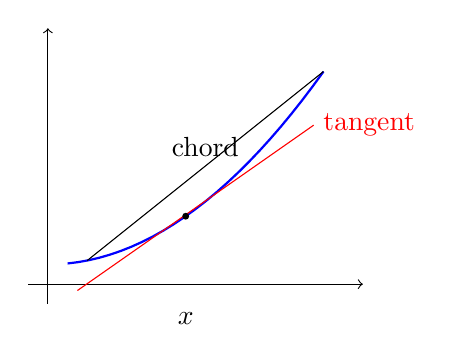
\begin{tikzpicture}[scale=1.25]
\draw[->] (-.2,0)--(3.2,0); \draw[->] (0,-.2)--(0,2.6);
\draw[blue,thick,domain=.2:2.8] plot(\x,{.25*\x*\x+.2});
\draw (.4,.24)--(2.8,2.16) node[midway,above] {chord};
\draw[red] (.3,-.065)--(2.7,1.615) node[right] {tangent};
\fill (1.4,.69) circle (.035);
\node at (1.4,-.35) {$x$};
\end{tikzpicture}
\end{center}
For $x<z<y$, the chord slope across $[x,y]$ is the weighted average
of the two smaller chord slopes, with weights $(z-x)/(y-x)$ and
$(y-z)/(y-x)$. Convexity orders the smaller slopes; their weighted
average lies between them. Passing to a tangent means taking a limit
of these ordered secant slopes.
\begin{theorem}[Derivative criteria for convexity]
\label{thm:convex-derivative-criteria}
Let $f$ be differentiable on an open interval $I$.  Then $f$ is convex if
and only if $f'$ is nondecreasing.  In that case every tangent line supports
the graph:
\[
f(y)\geq f(x)+f'(x)(y-x)
\qquad(x,y\in I).
\]
If $f''$ exists throughout $I$ and $f''\geq0$, then $f$ is convex.
\end{theorem}
\begin{proof}
For $x<z<y$, convexity at $z$ rearranges to
\[
\frac{f(z)-f(x)}{z-x}\leq\frac{f(y)-f(x)}{y-x}
\leq\frac{f(y)-f(z)}{y-z}.
\]
Keep $x,y$ fixed. Let $z\downarrow x$ in the left inequality and
$z\uparrow y$ in the right one to get
\[
f'(x)\leq\frac{f(y)-f(x)}{y-x}\leq f'(y).
\]
In particular $f'$ is nondecreasing. The first bound gives
$f(y)\geq f(x)+f'(x)(y-x)$ for $y>x$. For $y<x$, apply the second
bound to the ordered pair $y<x$ and rearrange to the same tangent inequality.

Conversely suppose $f'$ is nondecreasing. For $x<y$ and $0<t<1$, put
$z=tx+(1-t)y$, so $x<z<y$. The Mean Value Theorem on $[x,z]$ and
$[z,y]$ supplies $\xi_1\in(x,z)$ and $\xi_2\in(z,y)$ with
\[
\frac{f(z)-f(x)}{z-x}=f'(\xi_1)\leq f'(\xi_2)
=\frac{f(y)-f(z)}{y-z}.
\]
Multiply by the positive denominators and collect the $f(z)$ terms:
$(y-x)f(z)\leq(y-z)f(x)+(z-x)f(y)$.
Since $(y-z)/(y-x)=t$ and $(z-x)/(y-x)=1-t$, this is the chord inequality.
The cases $t=0,1$ are equalities; reversing $x,y$ covers the other order.
Finally, if $f''\geq0$, applying the Mean Value Theorem to $f'$ shows
that $f'$ is nondecreasing, so the result applies.
\end{proof}

Thus $x^2$, $e^x$, and $-\log x$ are convex on their natural domains, by
their nonnegative second derivatives.  The function $-x^2$ is not convex;
at the midpoint of $-1$ and $1$ its value $0$ lies above the chord value
$-1$.  Applying the tangent inequality to $e^x$ at $0$ gives the useful
estimate
\[
e^y\geq1+y.
\]

\begin{example}[A continuous trigonometric series]
For $0<a<1$ and any positive integer $b$, the series
\[
W(x)=\sum_{n=0}^\infty a^n\cos(\pi b^n x)
\]
converges uniformly on $\R$ by the bound $|a^n\cos(\pi b^nx)|\leq a^n$.
Its sum is therefore continuous. This argument establishes only continuity;
it proves no assertion about differentiability of this family. The formal
derivative terms have bounds $\pi(ab)^n$, which supply no convergent
geometric majorant when $ab\geq1$. Failure of this bound is not itself a
proof of nondifferentiability. To separate continuity from differentiability
within results proved here, recall $|x|$: its one-sided slopes at zero
are $-1$ and $1$, so it is continuous there but not differentiable.
\end{example}



\section*{Exercises}
\addcontentsline{toc}{section}{Exercises}

\begin{hexercise}{derivative-definition}
Prove from the difference quotient that $(1/x)^{\prime}=-1/x^2$ for $x\ne0$. Give denominator control explicitly. For the function equal to $x^2$ on $x\geq0$ and $cx$ on $x<0$, determine all $c$ for differentiability at zero.
\end{hexercise}

\begin{exercise}
Differentiate $(x^2+1)\exp x$, $\sin(x^2)$, $\log(1+x^2)$, and $(x+1)/(x^2+1)$. State domains and identify the rule used at each step.
\end{exercise}

\begin{exercise}
Evaluate $\sin(2x)/x$, $(\exp(3x)-1)/x$, $\log(1+2x)/x$, and $(1-\cos(2x))/x^2$ as $x\to0$, using the established elementary limits.
\end{exercise}

\begin{hexercise}{optimization-model}
A rectangle is made with $20$ metres of boundary. Determine its largest area. Formulate the variable, objective, and domain; identify all candidates and justify a global maximum.
\end{hexercise}

\begin{exercise}
A position is $s(t)=t^3$ metres for $0\leq t\leq2$ seconds. Find its average velocity and a time when the instantaneous velocity equals it. State the theorem hypotheses and give a uniform sensitivity bound for position errors caused by time errors.
\end{exercise}

\begin{exercise}
Use Taylor\textquotesingle s theorem to approximate $\exp(0.1)$ by $1+0.1+0.1^2/2$ and prove an error bound using $\exp(t)\leq\exp(1)$ on $[0,0.1]$.
\end{exercise}

\begin{exercise}
Use the Mean Value Theorem to prove that if
\[
\abs{f'(x)}\leq M
\qquad(x\in(a,b)),
\]
where $f$ is continuous on $[a,b]$ and differentiable on $(a,b)$, then
\[
\abs{f(y)-f(x)}\leq M\abs{y-x}
\qquad(x,y\in[a,b]).
\]
\end{exercise}

\begin{exercise}
Use \cref{thm:power-series-differentiation} to differentiate
\[
\sum_{n=0}^{\infty}(x-1)^n
\]
on its interval of convergence. Explain why this is an analytic theorem rather than merely a formal manipulation of symbols.
\end{exercise}

\begin{exercise}
Prove from the definitions that
\[
\arcsin(-x)=-\arcsin(x)
\qquad(-1\leq x\leq1).
\]
\end{exercise}

\begin{exercise}
For $F_n(x)=x+x^2/n$ on $[-1,1]$, verify the sequence differentiation
theorem including the anchor. Then explain why $F_n(x)=n+x$ fails it
despite uniformly convergent derivatives.
\end{exercise}
\begin{hexercise}{log-taylor}
Use the degree-two Taylor polynomial of $\log(1+x)$ at zero to
approximate $\log(1.1)$ with an explicit third-derivative error bound.
\end{hexercise}
\begin{exercise}
If all derivatives of a smooth function vanish at zero, must it vanish
near zero? Give a counterexample. What changes if it is analytic there?
\end{exercise}
% This final two-line exercise needs only three lines of reserved space.
\begingroup
\let\usualNeedspace\Needspace
\renewcommand{\Needspace}[1]{\usualNeedspace{3\baselineskip}}
\begin{exercise}
Use a supporting tangent line to prove $\log x\leq x-1$ for $x>0$.
State precisely which function is convex or concave in your argument.
\end{exercise}
\endgroup
